%%%%%%%%%%%%%%%%%%%%%%%%%%%%%%%%%%%%

\section{1.7.Dados categóricos}

%%%%%%%%%%%%%%%%%%%%%%%%%%%%%%%%%%%%

\subsection{Tabelas de Contingência e Gráficos de Barras}

%%%%%%%%%%%%%%%%%%%%%%%%%%%%%%%%%%%%

\begin{frame}
\frametitle{Tabelas de contingência}

\justifying
Uma tabela que resume a informação de duas variáveis categóricas é chamada de \hl {tabela de contingência}.

$\:$ \\
\pause
\justifying
A tabela de contingência abaixo mostra a distribuição dos gêneros dos alunos e se eles estão ou não procurando algum tipo de relacionamento durante a graduação.

\begin{center}
\begin{tabular}{l l cc rr}
					& 			& \multicolumn{2}{c}{{Procurando}} \\
  \cline{3-4}
					&			& Não	& Sim	& Total & \hspace{3mm}  \\ 
  \cline{2-5}
\multirow{2}{*}{{Gênero}}& Feminino 		& 86 	& 51 		& 137 \\ 
  					& Masculino 		& 52 	& 18	 	& 70\\ 
  \cline{2-5}
  					& Total		& 138& 69	&  207 \\
  \cline{2-5}
\end{tabular}
\end{center}

\end{frame}

%%%%%%%%%%%%%%%%%%%%%%%%%%%%%%%%%%%%

\begin{frame}
\frametitle{Gráficos de Barras}
\justifying
Um \hl {gráfico de barras} é uma maneira comum de exibir uma única variável categórica. Um gráfico de barras onde as proporções, em vez de frequências, são mostradas é chamado de \hl {barra de frequência relativa}.

\begin{center}
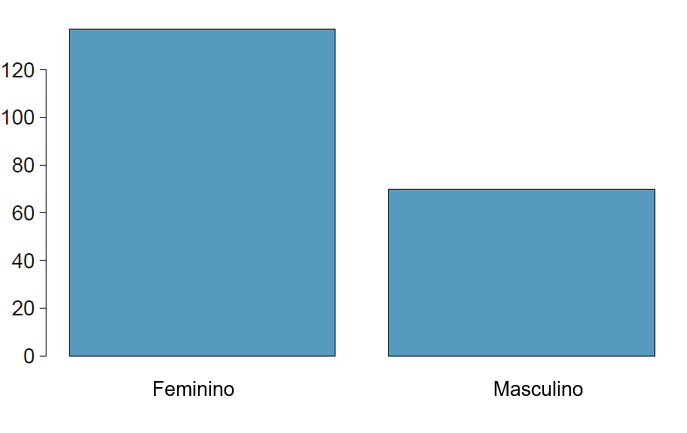
\includegraphics[width=0.45\textwidth]{1-7_categorical_data/gender_bar.png}
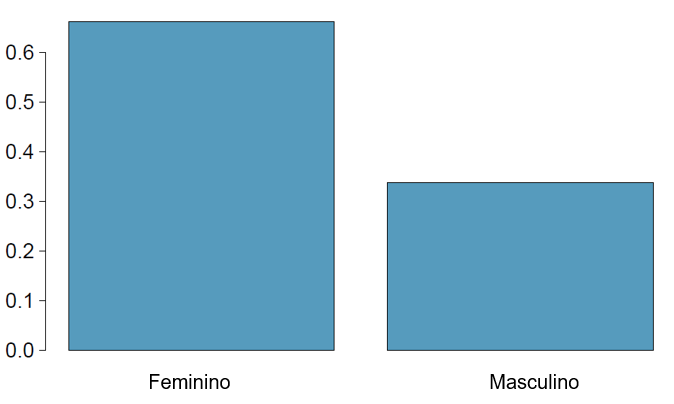
\includegraphics[width=0.45\textwidth]{1-7_categorical_data/gender_rel_bar.png}
\end{center}

\end{frame}
%%%%%%%%%%%%%%%%%%%%%%%%%%%%%%%%%%%%

\begin{frame}
\frametitle{Gráficos de Barras}
\dq{Qual a diferença entre gráfico de barras e histogramas?}
\justifying
\soln{\pause{{Gráficos de barra são usados para exibir distribuições de variáveis categóricas, enquanto histogramas são usados para variáveis numéricas. O eixo x em um histograma é uma linha numérica, portanto a ordem das barras não pode ser alterada, enquanto em um gráfico de barras as categorias podem ser listadas em qualquer ordem (embora algumas ordenações façam mais sentido que outras, especialmente para variáveis ordinais).
}}}

\end{frame}

%%%%%%%%%%%%%%%%%%%%%%%%%%%%%%%%%%

%%%%%%%%%%%%%%%%%%%%%%%%%%%%%%%%%%%%

\subsection{Proporções de linha e coluna}

%%%%%%%%%%%%%%%%%%%%%%%%%%%%%%%%%%%%

\begin{frame}
\frametitle{Escolhendo a proporção apropriada}
\justifying
\dq{Parece haver uma relação entre gênero e se o aluno está procurando algum relacionamento?}

\begin{center}
\begin{tabular}{l l cc r}
					& 			& \multicolumn{2}{c}{{Procurando }} \\
  \cline{3-4}
					&			& Não	& Sim	& Total \\ 
  \cline{2-5}
\multirow{2}{*}{{Gênero}}& Feminino 		& 86 	& 51 		& 137 \\ 
  					& Masculino 		& 52 	& 18	 	& 70\\ 
  \cline{2-5}
  					& Total		& 138& 69	&  207 \\
  \cline{2-5}
\end{tabular}
\end{center}

\pause
\justifying
Para responder a essa pergunta, examinamos as proporções nas linhas: 

\pause

\begin{itemize}
\justifying
\item \% Mulheres à procura de um relacionamento: $51 / 137 \approx 0.37$ \\

\pause
\justifying
\item \% Homens procurando por um relacionamento: $18 / 70 \approx 0.26$ \\

\end{itemize}

\end{frame}

%%%%%%%%%%%%%%%%%%%%%%%%%%%%%%%%%%%%

\subsection{Barras segmentadas e mosaicos}

%%%%%%%%%%%%%%%%%%%%%%%%%%%%%%%%%%%%

\begin{frame}
\frametitle{Barras segmentadas e mosaicos}
\justifying
\dq{Abaixo os gráficos respresentando a tabela do slide anterior. Quais são as diferenças entre as três visualizações mostradas abaixo?}

\begin{center}
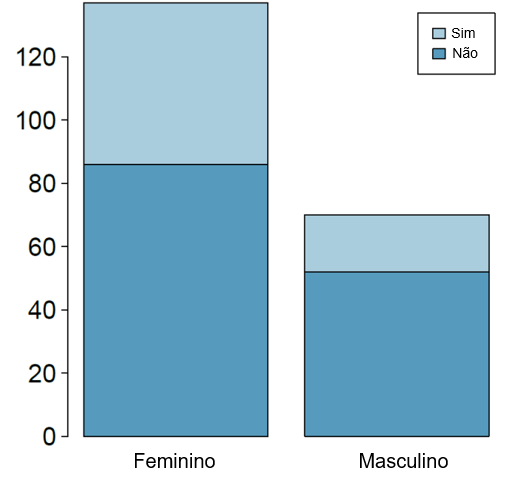
\includegraphics[width=0.33\textwidth]{1-7_categorical_data/gender_seg_bar.png}
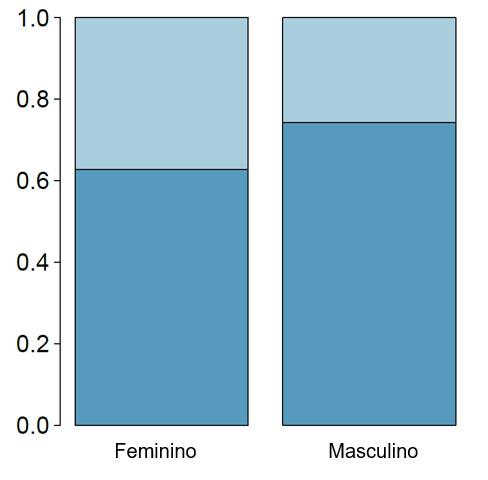
\includegraphics[width=0.33\textwidth]{1-7_categorical_data/gender_rel_seg_bar.png}
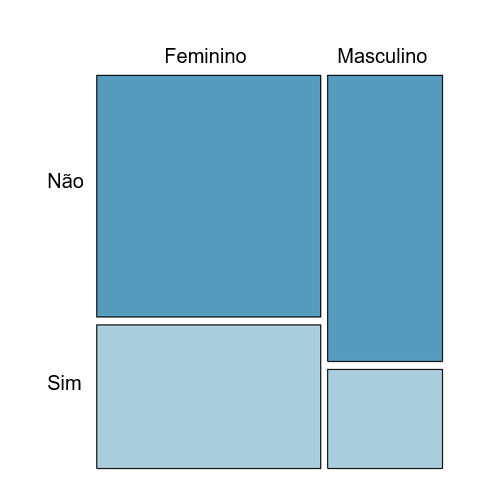
\includegraphics[width=0.33\textwidth]{1-7_categorical_data/gender_mosaic.png}
\end{center}

\end{frame}

%%%%%%%%%%%%%%%%%%%%%%%%%%%%%%%%%%%%

\subsection{Gráfico de setores}

%%%%%%%%%%%%%%%%%%%%%%%%%%%%%%%%%%%%

\begin{frame}
\frametitle{Gráfico de setores}
\justifying
\dq{Você pode dizer qual grupo engloba a menor porcentagem de espécies de mamíferos?}

\vspace{-0.5cm}

\begin{center}
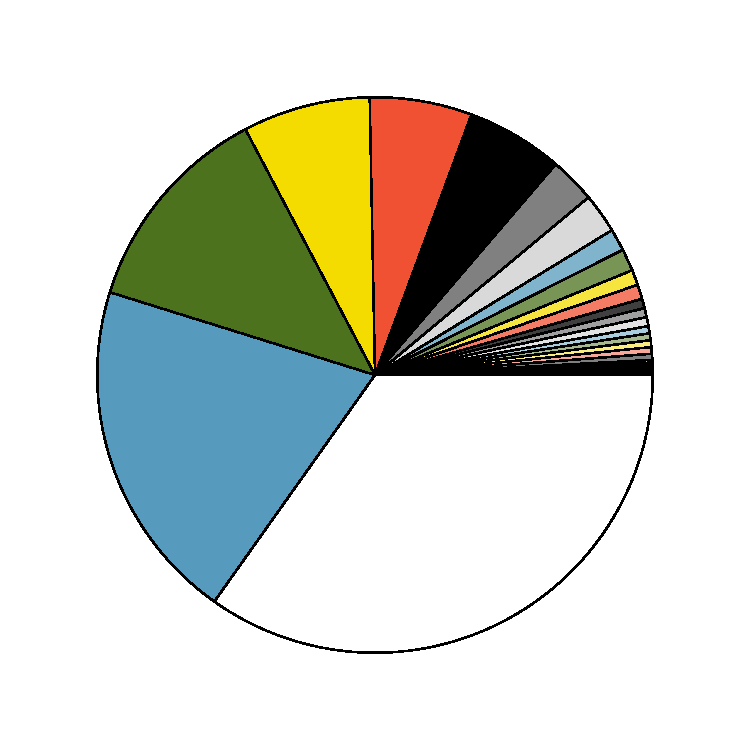
\includegraphics[width=0.4\textwidth]{1-7_categorical_data/mammal_pie_chart.pdf}
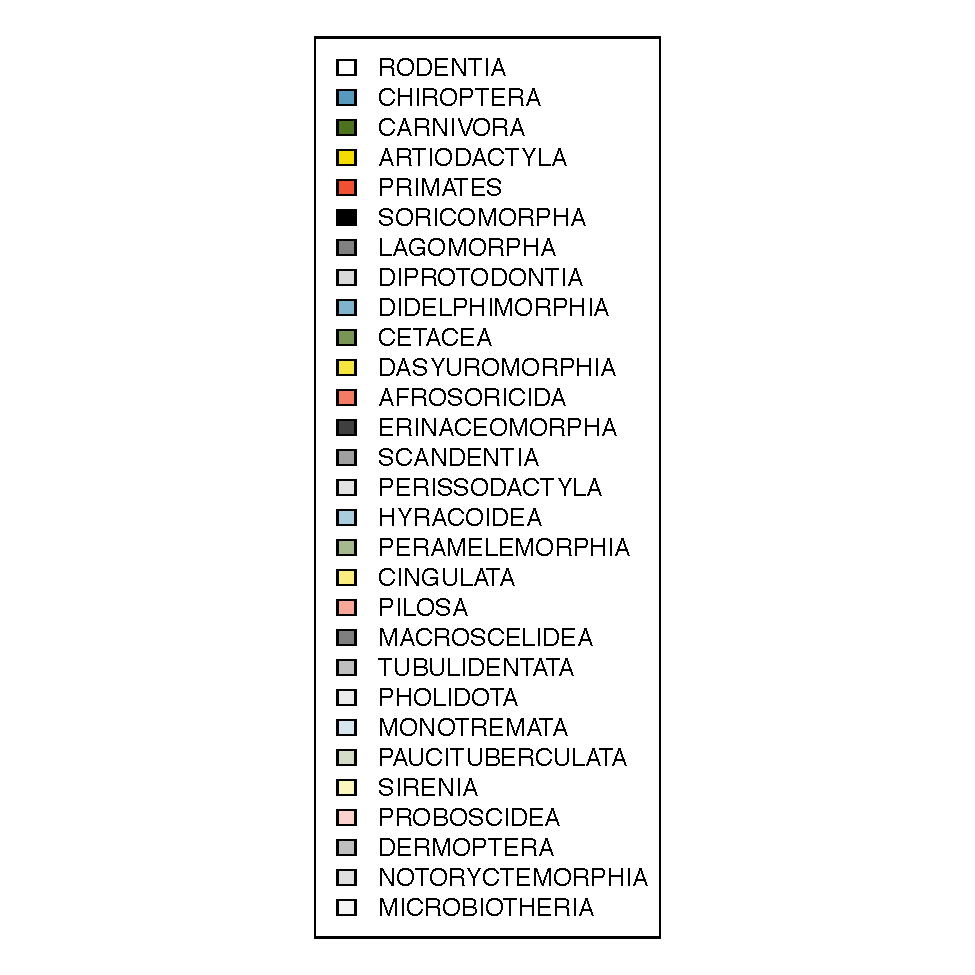
\includegraphics[width=0.2\textwidth]{1-7_categorical_data/mammal_pie_chart_legend.pdf}
\end{center}
\justifying
\ct{Dados de \webURL{http://www.bucknell.edu/msw3}.}

\end{frame}


%%%%%%%%%%%%%%%%%%%%%%%%%%%%%%%%%%%%

\subsection{Comparando dados numéricos entre grupos}

%%%%%%%%%%%%%%%%%%%%%%%%%%%%%%%%%%%%

\begin{frame}
\frametitle{Gráfico de boxplot lado a lado}
\justifying
\dq{Parece haver uma relação entre o ano da turma e o número de clubes frequentados pelos alunos?}

\begin{center}
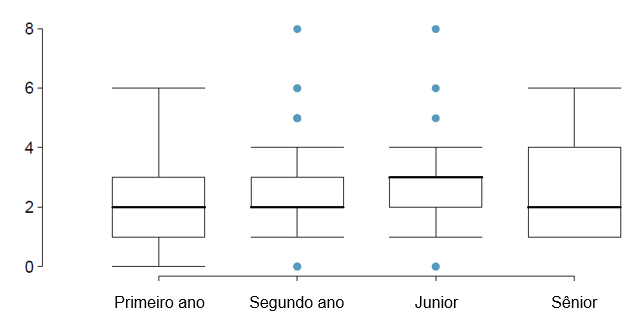
\includegraphics[width=\textwidth]{1-7_categorical_data/year_clubs.png}
\end{center}
%%%%MUDARRR
\end{frame}

%%%%%%%%%%%%%%%%%%%%%%%%%%%%%%%%%%%%


